%%%%%%%%%%%%%%%%%%%%%%%%%%%%%%%%%%%
%%%%%%%%%%%%%%%%%%%%%%%%%%%%%%%%%%%
\begin{frame}
  \frametitle{Programming with structured parallel patterns}

  \begin{minipage}{0.7\linewidth}
    \begin{itemize}
    \item \textcolor{red}{\textbf{pattern}} : \textbf{a basic structural entity of an algorithm}
      % http://parallelbook.com/sites/parallelbook.com/files/SC13_20131117_Intel_McCool_Robison_Reinders_Hebenstreit.pdf
    \item book \myhref{http://parallelbook.com/}{Structured Parallel Programming:} \myhref{http://parallelbook.com/}{Patterns for Efficient Computation}
    \end{itemize}
  \end{minipage}
  \hfill{}
  \begin{minipage}{0.25\linewidth}
    \vfill{}
    %\begin{center}
    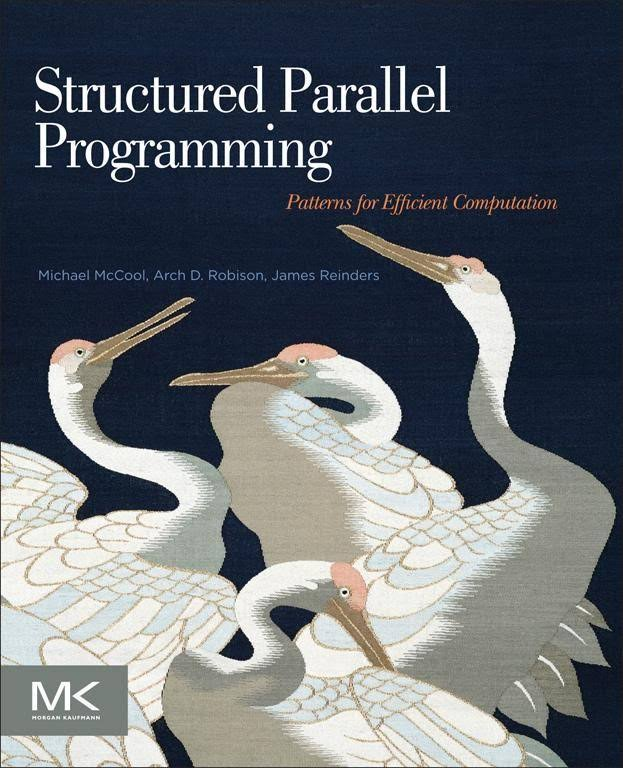
\includegraphics[width=2.5cm]{images/structured_parallel_programming}
    %\end{center}
  \end{minipage}

  \begin{itemize}
    \item implementation: Intel TBB, OpenMP, OpenACC and many others
    \item  {\small \myhref{https://sharepoint.campus.rwth-aachen.de/units/rz/HPC/public/Shared\%20Documents/WienkeEtAl_OpenACC-OpenMP-PatternComparison.pdf}{OpenMP/OpenAcc for GPU/XeonPhi: pattern-based comparison}: map, stencil, reduce, scan, fork-join, superscalar sequence, parallel update}
      % map -> SAXPY
  \end{itemize}

  {\scriptsize
  reference:\\
  \myhref{http://link.springer.com/chapter/10.1007/978-3-319-09873-9_68}{A Pattern-Based Comparison of OpenACC and OpenMP for Accelerator Computing}}

\end{frame}

%%%%%%%%%%%%%%%%%%%%%%%%%%%%%%%%%%%
%%%%%%%%%%%%%%%%%%%%%%%%%%%%%%%%%%%
\begin{frame}
  \frametitle{Programming with structured parallel patterns}

  \begin{center}
  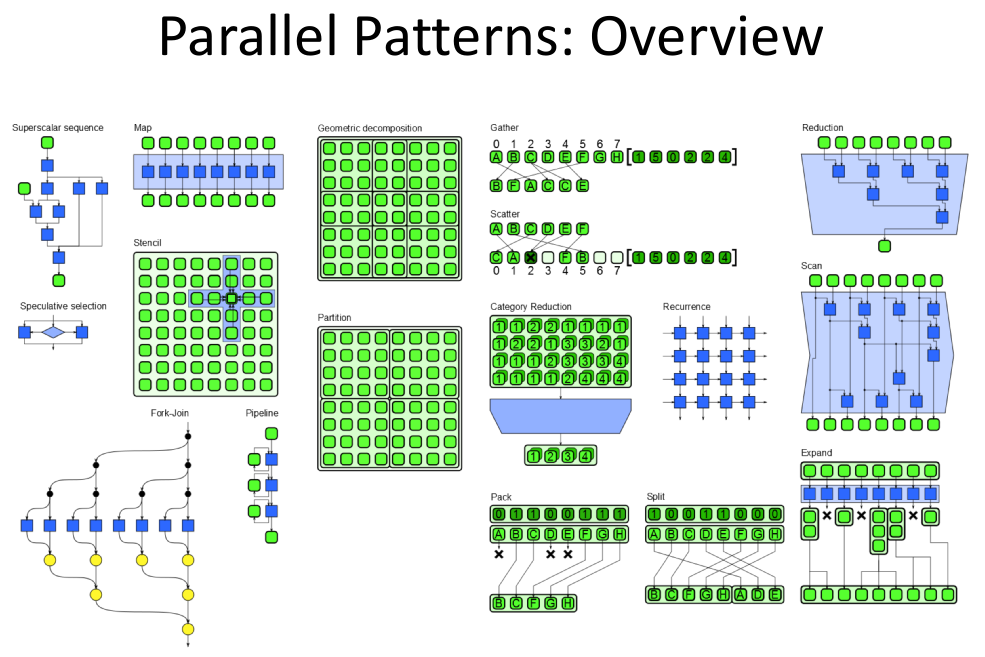
\includegraphics[width=9cm]{images/parallel_patterns2}
  \end{center}

  {\scriptsize
  reference: Structured Parallel Programming with Patterns, SC13 tutorial, by M. Hebenstreilt, J. reinders, A. Robison, M. McCool}

\end{frame}
